\documentclass[10pt]{beamer}
\usetheme[
%%% option passed to the outer theme
%    progressstyle=fixedCircCnt,   % fixedCircCnt, movingCircCnt (moving is deault)
  ]{Feather}
  
% If you want to change the colors of the various elements in the theme, edit and uncomment the following lines

% Change the bar colors:
%\setbeamercolor{Feather}{fg=red!20,bg=red}

% Change the color of the structural elements:
%\setbeamercolor{structure}{fg=red}

% Change the frame title text color:
%\setbeamercolor{frametitle}{fg=blue}

% Change the normal text color background:
%\setbeamercolor{normal text}{fg=black,bg=gray!10}

%-------------------------------------------------------
% INCLUDE PACKAGES
%-------------------------------------------------------

\usepackage[utf8]{inputenc}
\usepackage[english]{babel}
\usepackage[T1]{fontenc}
\usepackage{helvet}

%-------------------------------------------------------
% DEFFINING AND REDEFINING COMMANDS
%-------------------------------------------------------

% colored hyperlinks
\newcommand{\chref}[2]{
  \href{#1}{{\usebeamercolor[bg]{Feather}#2}}
}

%-------------------------------------------------------
% INFORMATION IN THE TITLE PAGE
%-------------------------------------------------------

\title[] % [] is optional - is placed on the bottom of the sidebar on every slide
{ % is placed on the title page
      \textbf{Control Systems EE2227}
}

\subtitle[EE2227 Control Systems]
{
      \textbf{Gate Problems (EE2017 SET 1 paper) }
}

\author[Shreshta Thumati]
{      Shreshta Thumati \\
      {\ttfamily EE18BTECH11041}
}

\institute[]
{
     
  
  %there must be an empty line above this line - otherwise some unwanted space is added between the university and the country (I do not know why;( )
}

\date{}

%-------------------------------------------------------
% THE BODY OF THE PRESENTATION
%-------------------------------------------------------

\begin{document}

%-------------------------------------------------------
% THE TITLEPAGE
%-------------------------------------------------------

{\1% % this is the name of the PDF file for the background
\begin{frame}[plain,noframenumbering] % the plain option removes the header from the title page, noframenumbering removes the numbering of this frame only
  \titlepage % call the title page information from above
\end{frame}}



%-------------------------------------------------------
\section{Question}
%-------------------------------------------------------
\subsection{}
\begin{frame}{Question}
%-------------------------------------------------------
In a system whose signal flow graph is shown in the figure, $U_1(s)$ and $U_2(s)$ are inputs. The transfer function $\dfrac{Y(s)}{U_1(s)}$ is
\begin{figure}
    \centering
    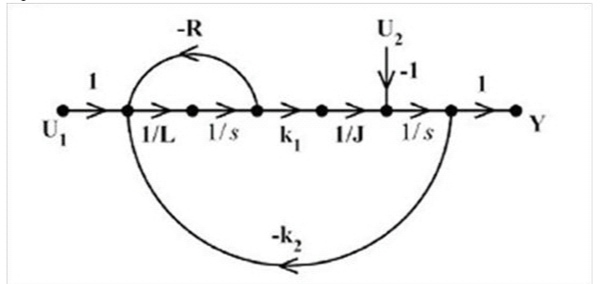
\includegraphics[width=7cm]{image.jpg}

\end{figure}


(a) {$\dfrac{k1}{JLs^2+ J R s+ k_1 k_2}$}
\hspace{2cm}
(b) {$\dfrac{k1}{JLs^2- J R s- k_1 k_2}$}

(c) {$\dfrac{k1-U_2(R+sL)}{JLs^2+(JR-U_2L)s+ k_1 k_2-U_2 R}$}

(d) {$\dfrac{k1-U_2(sL-R)}{JLs^2-(JR+U_2L)s- k_1 k_2+U_2 R}$}

\end{frame}


%-------------------------------------------------------
\section{Solution}
%-------------------------------------------------------
\subsection{}
\begin{frame}{Solution}
%-------------------------------------------------------
Masons Gain Formula:

$T=\dfrac{C(s)}{R(s)}=\dfrac{\sum_{i=1}^{N}P_i \Delta_i }{\Delta}$

where,
\begin{itemize}
    \item T is the transfer function or the gain between R(s) and C(s)
    \item C(s) is the output node
    \item R(s) is the input node
    \item $P_i$ is the i\textsuperscript{th} forward path gain
    \item $\Delta= 1 - $(sum of all individual loop gains)+(sum of gain products of all possible two non touching loops)-(sum of gain products of all possible three non touching loops)+.... 
    \item $\Delta_i$ is obtained from $\Delta$ by removing the loops which are touching the i\textsuperscript{th} forward path  
     
    
    
\end{itemize}


\end{frame}


%-------------------------------------------------------
\section{Solution}
%-------------------------------------------------------
\subsection{}
\begin{frame}{Solution}
%-------------------------------------------------------
\begin{figure}
    \centering
    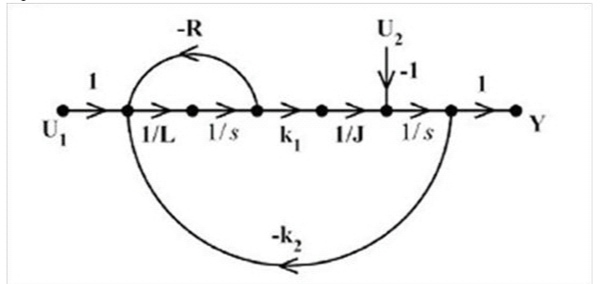
\includegraphics[width=7cm]{image.jpg}

\end{figure}

\[
\dfrac{Y(s)}{U_1(s)}\Biggr|_{U_2(s)=0}
\]
\[
P_1=1\cdot\dfrac{1}{L}\cdot\dfrac{1}{s}\cdot k_1 \cdot\dfrac{1}{J}\cdot\dfrac{1}{s}\cdot1=\dfrac{k_1}{LJs^2}
\]


\end{frame}

%-------------------------------------------------------
\section{Solution}
%-------------------------------------------------------
\subsection{}
\begin{frame}{Solution}
%-------------------------------------------------------
\begin{figure}
    \centering
    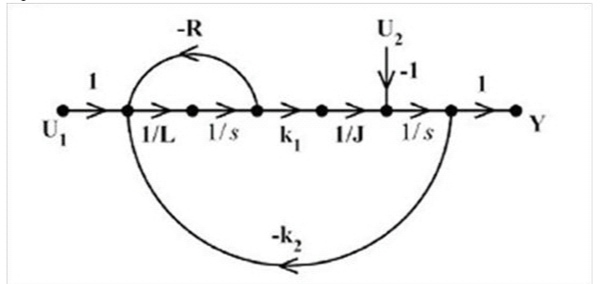
\includegraphics[width=7cm]{image.jpg}

\end{figure}

\[ \Delta_1 =1
\]
After removing the loops that are touching the forward path, the system will have no loops .Therefore, $\Delta_1$ will be 1.


\end{frame}

%-------------------------------------------------------
\section{Solution}
%-------------------------------------------------------
\subsection{}
\begin{frame}{Solution}
%-------------------------------------------------------
\begin{figure}
    \centering
    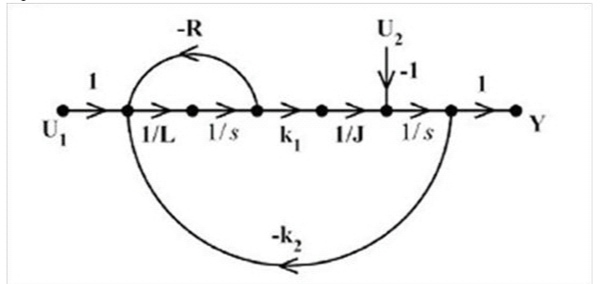
\includegraphics[width=7cm]{image.jpg}

\end{figure}

$\Delta= 1 - $(sum of all individual loop gains)
as in this system there are no non touching loops.
Let $L_1$ and $L_2$ be the individual loops.

\centering
$\Delta= 1 - (L_1+L_2)$
\[

L_1= \dfrac{1}{L}\cdot \dfrac {1}{s}\cdot(-R)=\dfrac{-R}{Ls}
\]

\[
L_2=\dfrac{1}{L}\cdot \dfrac{1}{s}\cdot k_1 \cdot \dfrac{1}{J} \cdot \dfrac{1}{s}\cdot -(k_2) =\dfrac{-k_2 k_1}{LJs^2}
\]

\end{frame}
%-------------------------------------------------------
\section{Solution}
%-------------------------------------------------------
\subsection{}
\begin{frame}{Solution}
%-------------------------------------------------------
\begin{figure}
    \centering
    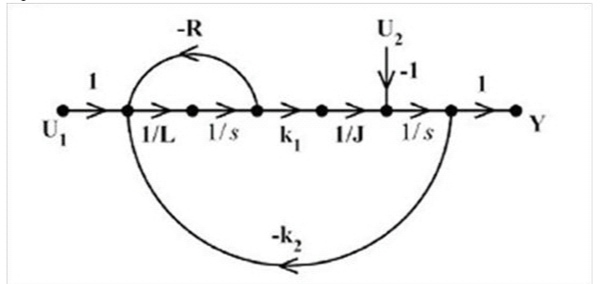
\includegraphics[width=7cm]{image.jpg}

\end{figure}
\begin{align}

P_1=\dfrac{k_1}{LJs^2} \hspace{0.75cm}
\Delta_1 =1 \hspace{0.75cm}
L_1=\dfrac{-R}{Ls}\hspace{0.75cm}
L_2=\dfrac{-k_2 k_1}{LJs^2}   

\end{align}

\[
\dfrac{Y(s)}{U_1(s)} = \dfrac{P_1 \Delta_1}{1-(L_1+L_2)}=\dfrac{\dfrac{k_1}{s^2LJ}}{1+\dfrac{R}{Ls}+\dfrac{k_2 k_1}{LJs^2}}
\]

\end{frame}

%-------------------------------------------------------
\section{Solution}
%-------------------------------------------------------
\subsection{}
\begin{frame}{Solution}
%-------------------------------------------------------
\begin{figure}
    \centering
    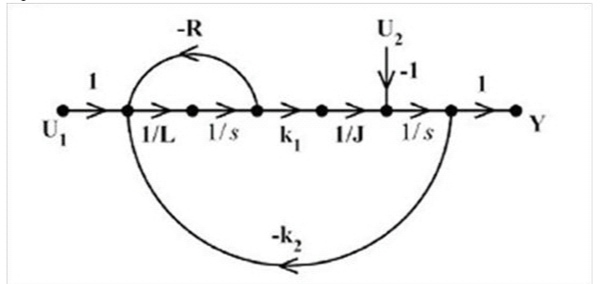
\includegraphics[width=7cm]{image.jpg}

\end{figure}
\centering
\[

 \dfrac{Y(s)}{U_1(s)}=\dfrac{k_1}{s^2LJ+sRJ+K_1k_2}

\]
\end{frame}




\end{document}